\documentclass[tikz,border=10pt]{standalone}
\usetikzlibrary{calc}
\begin{document}
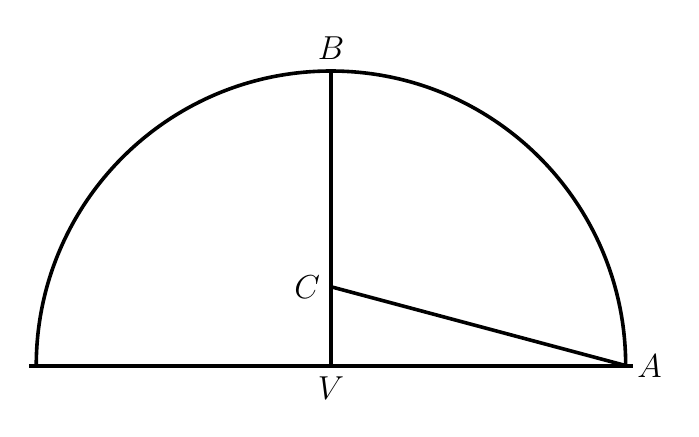
\begin{tikzpicture}[line width=1.3pt, line join=round,
  every node/.style={font=\fontsize{13}{15.6}\selectfont}]
% Units: cm, scale s = 0.015873 (longest side 8 cm), origin at centre V
\coordinate (V) at (0,0);
\coordinate (A) at (3.751,0);        % right end of diameter
\coordinate (D) at (-3.829,0);       % left end of diameter (x=23 px)
\coordinate (E) at (3.838,0);        % right end of diameter (x=506 px)
\coordinate (B) at (0,3.748);        % apex
\coordinate (C) at (0,1.003);        % point on BV
\coordinate (P) at (-3.743,0);       % left endpoint of semicircle, radius 3.743

% Upper semicircle (solid, no lower half)
\draw ($(V)+(180:3.743)$) arc[start angle=180, end angle=0, radius=3.743];

% Horizontal diameter
\draw (D) -- (E);

% Vertical segment B-V (C lies on it, so CV is not drawn separately)
\draw (B) -- (V);

% Segment A-C
\draw (A) -- (C);

% Labels
\node[right] at (A) {$A$};           % A label: right of vertex, level with it
\node[above] at (B) {$B$};
\node[left] at (C) {$C$};
\node[below] at (V) {$V$};           % V label: centred directly below
\end{tikzpicture}
\end{document}